\texttt{•}% Chapter 1

\chapter{Introducción general} % Main chapter title
\label{Chapter1} % For referencing the chapter elsewhere, use \ref{Chapter1} 
\label{IntroGeneral}

%----------------------------------------------------------------------------------------

% Define some commands to keep the formatting separated from the content 
\newcommand{\keyword}[1]{\textbf{#1}}
\newcommand{\tabhead}[1]{\textbf{#1}}
\newcommand{\code}[1]{\texttt{#1}}
\newcommand{\file}[1]{\texttt{\bfseries#1}}
\newcommand{\option}[1]{\texttt{\itshape#1}}
\newcommand{\grados}{$^{\circ}$}

%----------------------------------------------------------------------------------------

%\section{Introducción}

%----------------------------------------------------------------------------------------
\section{Inteligencia Artificial, Aprendizaje Automatico y Aprendizaje Profundo}

AI (\textit{Artificial Intelligence}, Intelegencia Artificial), ML (\textit{Machine Learning}, Aprendizaje Automatico) y DL (\textit{Deep Learning}, Aprendizaje Profundo), son terminos muy utilizados hoy en dia en el mundo del desarrollo tecnologico [ref]. Aunque estos terminos son muy parecidos, entre ellos existen dependencias que pueden ser visulizadas con ayuda de la figura \ref{fig:ai_ml_dl}.

\begin{figure}[h]
	\centering
	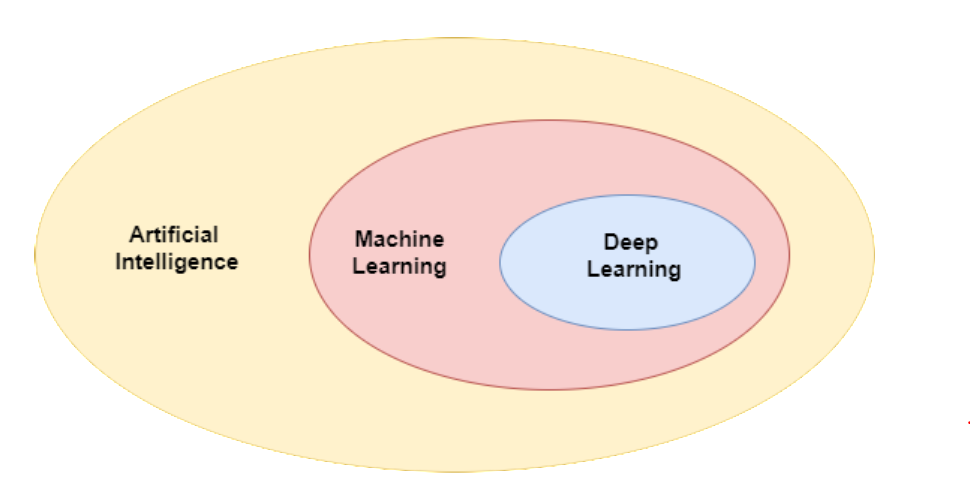
\includegraphics[scale=0.3]{./Figures/ai_ml_dl.png}
	\caption{Diferencias entre AI, ML y DL.}
	\label{fig:ai_ml_dl}
\end{figure}

AI es un area de la computacion que permite a los sistemas computacionales imitar la inteligencia humana para entender su entorno y tomar acciones que maximicen sus posibilidades de lograr sus objetivos [ref]. Sus aplicaciones más importante se ecuentran en la áreas de comercio, educación, robótica, salud, agricultura, automotriz y finanzas[https://www.simplilearn.com/tutorials/artificial-intelligence-tutorial/artificial-intelligence-applications]. Todos los sistemas de inteligencia artificial reales e hipotéticos pueden ser clasificados en alguno de los siguientes tipos:
\begin{itemize}
	\item ANI (\textit{Artificial Narrow Intelligence, Inteligencia Artificial Estrecha}): también conocida como inteligencia artificial débil, su objetivo es llevar a cabo un solo tipo de tarea. Estos sistemas no poseen consciencia y no son manejados por sentimientos como lo haría un humano. Algunos ejemplos de ANI son los chat bots o los automóviles autónomos.
	\item AGI (\textit{Artificial General Intelligence}, Inteligencia Artificial General): también conocida como inteligencia artificial fuerte, es un concepto en el que las máquinas exhiben inteligencia humana. Estos sistemas tendrían la capacidad de aprender, entender y actuar de tal manera que sería indistinguible a un humano. AIG actualmente no existe, pero es utilizado en industrias como el cine 
	\item ASI (\textit{Artificial Super Intelligence}, Super Inteligencia Artificial): ASI también forma parte de la inteligencia artificial fuerte. Se le considera muy poderosa por ser capaz de volverse consciente y autónoma.
No solo replica el comportamiento humano, sino que lo supera. Puede pensar mejor y tener más habilidades. Sin embargo, esta tecnología aún está en desarrollo.
\end{itemize}

ML es un subconjunto de AI que utiliza algoritmos de aprendizaje estadísticos para contruir sistemas con la habilidad de aprender automáticamente y mejorar a partir de experiencias previas sin ser explícitamente programados para esto. Muchos de los servicios de recomendación utilizados por empresas con Netflix, YouTube o Spotify, utilizan ML para adapatarse a un usuario en particular y ofrecer una mejor experiencia más personalizada. Estos algoritmos pueden ser clasificados de la siguiente manera:
\begin{itemize}
	\item Aprendizaje supervisado: se refiere al aprendizaje modelos a partir de un conjunto de datos, mejor conocidos como \textit{dataset}, cuyas respuestas son conocidas con antelación y están asociadas a una etiqueta o \textit{label}. Por ejemplo, el \textit{dataset} pueden ser muchas fotografías de gatos y el \textit{label} asociado el nombre de este animal. De esta manera el modelo es entrenado para generar predicciones de datos nuevos. En la figura \ref{fig:ml_sl} se representa gráficamente el aprendizaje supervisado.
	\begin{figure}[h]
		\centering
		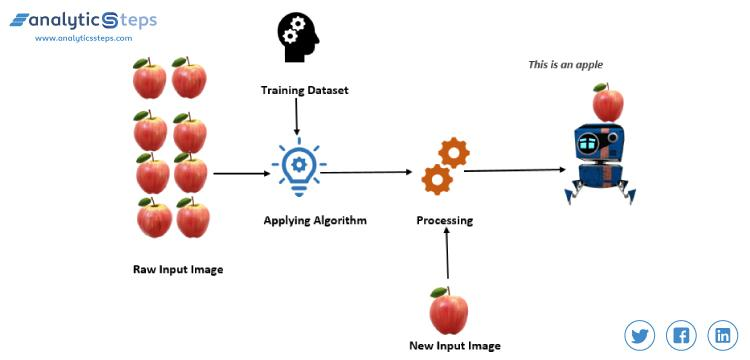
\includegraphics[scale=0.4]{./Figures/ml_sl.jpg}
		\caption{Aprendizaje supervisado.}
		\label{fig:ml_sl}
	\end{figure}
	
	\item Aprendizaje no supervisado: es utilizado cuando los datos utilizados para el aprendizaje no tienen \textit{labels}. Su objetivo principal es aprender acerca de los datos e inferir patrones sin ningún tipo de referencia sobre las respuestas esperadas. Es mayormente utilizado como parte del análisis exploratorio de datos [https://towardsdatascience.com/understanding-the-difference-between-ai-ml-and-dl-cceb63252a6c]. En la figura \ref{fig:ml_ul} se representa gráficamente el aprendizaje no supervisado.
	\begin{figure}[h]
		\centering
		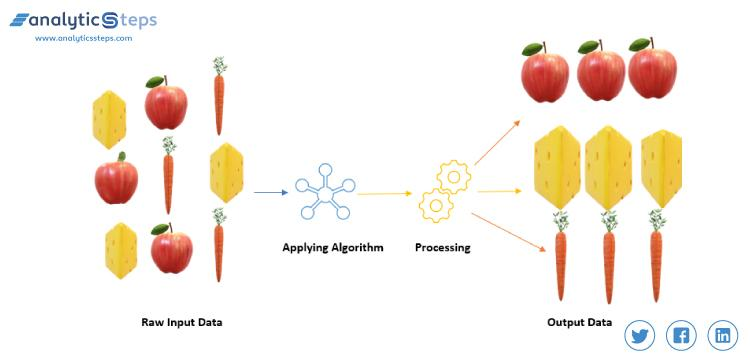
\includegraphics[scale=0.4]{./Figures/ml_ul.jpg}
		\caption{Aprendizaje no supervisado.}
		\label{fig:ml_ul}
	\end{figure}
	\item Aprendizaje reforzado: es el aprendizaje mediante la interacción continua con el entorno con el método de prueba y error, y utiliza continuamente la retroalimentación de sus acciones y experiencias previas. Este tipo de aprendizaje utiliza recompensas si se realizan acciones correctas y penalizaciones si son incorrectas. En la figura \ref{fig:ml_rl} se representa gráficamente el aprendizaje reforzado.
	\begin{figure}[h]
		\centering
		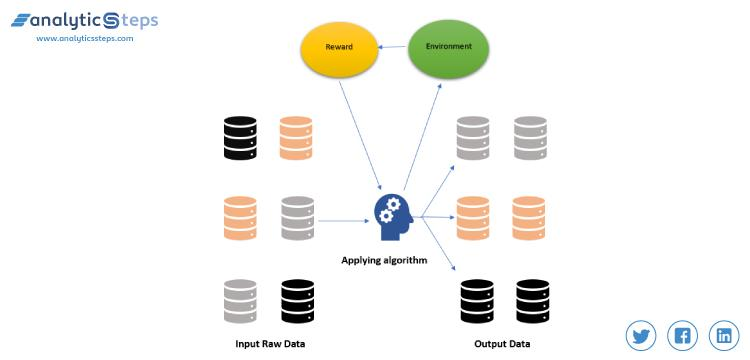
\includegraphics[scale=0.4]{./Figures/ml_rl.jpg}
		\caption{Aprendizaje reforzado.}
		\label{fig:ml_rl}
	\end{figure}
\end{itemize}

DL es una técnica de ML  que está inspirada en la forma en la que el cerebro humano filtra información. Como DL procesa información de manera similar al cerebro humano sus aplicaciones son tareas que un humano generalmente realiza, como distinguir entre un peatón o un poste de luz en el caso de automóviles autónomos. El componente principal de DL son las redes neuronales artificiales, que son capas de nodos interconectadas, donde existen una capa de entrada, una o varias capas ocultas y una capa de salida. En la figura \ref{fig:neural_network} se puede observar la arquitectura de una red neuronal artificial.
\begin{figure}[h]
	\centering
	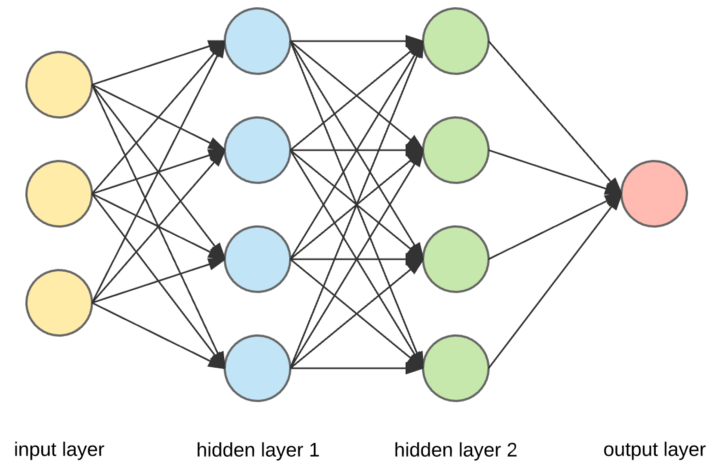
\includegraphics[scale=0.4]{./Figures/neural_network.png}
	\caption{Arquitectura de una red neuronal artificial.}
	\label{fig:neural_network}
\end{figure}

Cada uno de los nodos de las capas ocultas y de salida, tienen como entrada la salida de los nodos anteriores multiplicadas por unos términos denominados pesos o \textit{weigths} y que sumados junto a otro término llamado sesgo o \textit{bias} pasan por una función de activación no lineal para generar su salida. En la figura \ref{fig:neural_network_node} se visualizar un nodo de las capas ocultas o de salida.
\begin{figure}[h]
	\centering
	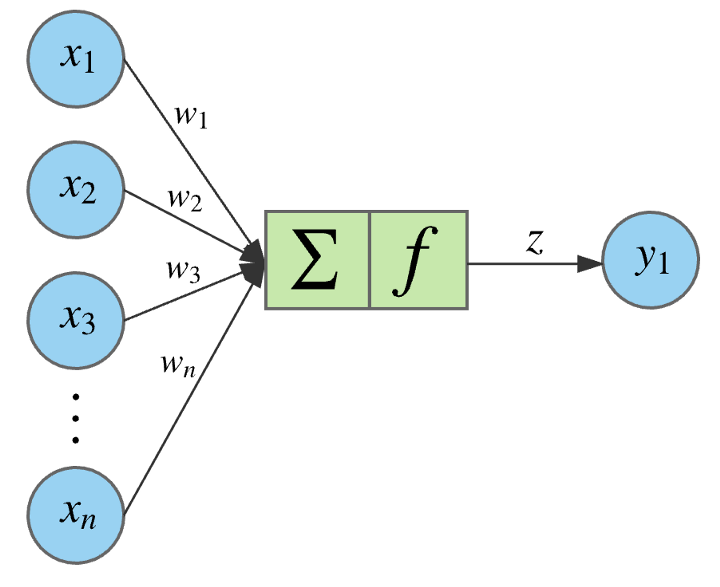
\includegraphics[scale=0.25]{./Figures/neural_network_node.png}
	\caption{Nodo de una red neuronal artificial.}
	\label{fig:neural_network_node}
\end{figure}

%----------------------------------------------------------------------------------------
\section{Redes neuronales convolucionales}
También conocidas como CNN (\textit{Convolutional Neural Networks}, Redes Neuronales Convolucionales) o ConvNet, son un algoritmo de DL que están orientadas a recibir como entrada una, asignarle \textit{weights} y \textit{biases} entrenables a varios aspectos/objetos en la imagen para poder diferenciarlas unas de otras. Su uso reduce el pre procesamiento de las imágenes de entrada con respecto a otros modelos de clasificación, ya que los filtros necesarios son incorporados en su arquitectura y tienen la habilidad de ser entrenados.

Computacionalmente una imagen puede ser muy dificil de procesar, esto depende del espacio de colores donde se encuentra [ref] y las dimensiones que posee. Por ejemplo una imagen RGB (\textit{Red Green Blue}, Rojo Verde Azul) y de dimensiones 1920x1080 pixeles, tiene un tamaño de 6220800 bytes. El objetivo principal de las CNN es reducir la dimensionalidad de las imágenes de entrada, de tal forma que sean más fáciles de procesar y no pierdan sus características o \textit{features} principales que son críticas para obtener una buena predicción.

La arquitectura de una CNN es independiente del tipo de aplicación, donde las capas que lo componen son elegidas en función de los objetivos que se persiguen. En la figura \ref{fig:cnn_arch} se puede observar la arquitectura de una CNN para clasificar digitos escritos a mano.

\begin{figure}[h]
	\centering
	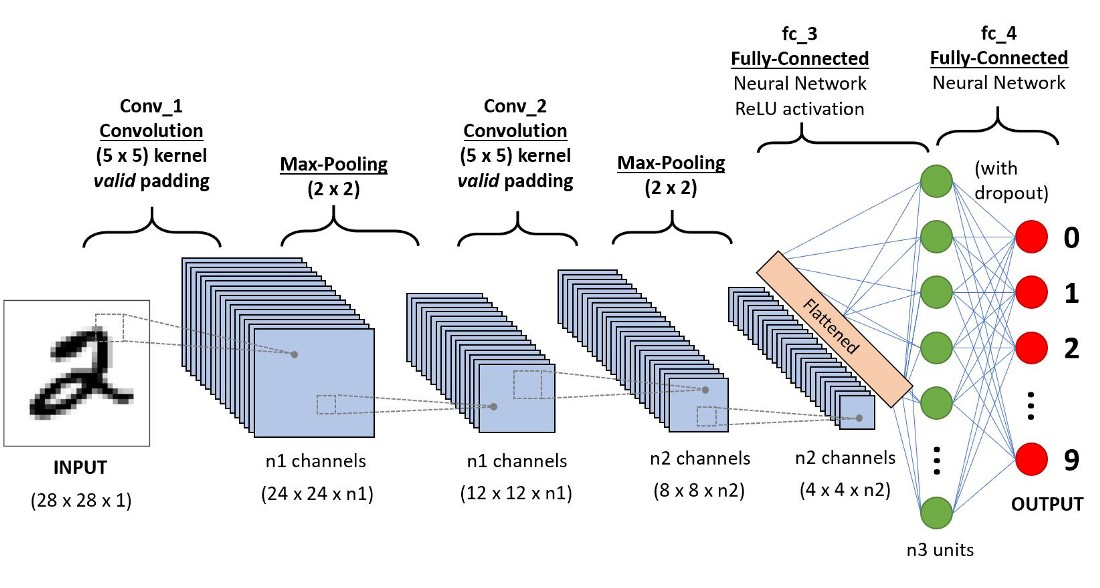
\includegraphics[scale=0.35]{./Figures/cnn_arch.jpeg}
	\caption{CNN para clasificar digitos escritos a mano.}
	\label{fig:cnn_arch}
\end{figure}

En la arquitectura de la figura \ref{fig:cnn_arch} se pueden observar tres capas principales para construir una CNN: capa de convoluciones, capa de \textit{pooling} y capa \textit{fully-connected}.

\subsection{Capa de convoluciones}
Esta capa esta encargada de aplicar la operación de convolución sobre las imágenes de entrada para encontrar patrones que más adelante permitirán clasificarla. La convolución de una imagen con un \textit{kernel} no es más que la aplicación del operador punto entre ambos. Este tipo de capas se definen por:´
\begin{itemize}
	\item El número de los \textit{kernels} o filtros que se aplican a la imagen, que es el número de matrices por las que se van a convolucionar las imágenes de entrada.
	\item El tamaño de los \textit{kernels}, donde casi siempre tienen dimensiones cuadradas e impares como 3x3 o 5x5.
	\item El \textit{stride} o paso, se refiere a la forma en como el \textit{kernel} recorre la imagen.
\end{itemize}

En la figura \ref{fig:cnn_conv} se puede observar como un 

\begin{figure}[h]
	\centering
	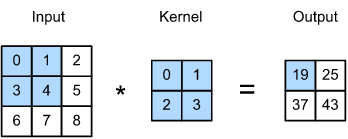
\includegraphics[scale=0.7]{./Figures/cnn_conv.png}
	\caption{Convolución de una entrada de 3x3 con un \textit{kernel} de 2x2 y \textit{stride} de 1.}
	\label{fig:cnn_conv}
\end{figure}

\subsection{Capa de \textit{pooling}}
Similar a la capa de convoluciones, tiene el objetivo de reducir la dimensionalidad de los \textit{features} obtenidos mediante las convoluciones aplicadas en la capa anterior, para reducir el poder computacional requerido en un principio. Existen dos tipos de dos tipos: \textit{max pooling} y \textit{Average pooling}. El primero retorna el valor maximo de una porcion de la imagen cubierta por el \textit{kernel} y el segundo el valor promedio o \textit{average}. \textit{Max pooling} tambien funciona como supresor de ruido al mismo tiempo que reduce la dimensionalidad. Mientras que \textit{average pooling} solo sirve para reducir la dimensionalidad. En la figura \ref{fig:cnn_pool} se pueden observar estos tipos de \textit{pooling}.

\begin{figure}[h]
	\centering
	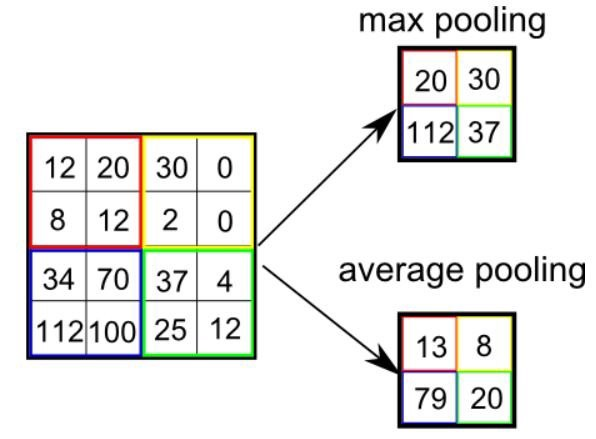
\includegraphics[scale=0.3]{./Figures/cnn_pool.png}
	\caption{Tipos de \textit{pooling}.}
	\label{fig:cnn_pool}
\end{figure}

\subsection{Capa \textit{fully-connected}}
Tambien conocida como capa lineal o FC (\textit{Fully Connected}, Totalmente Conectada), es simplemente una red neuronal artificial como la
mostrada en la seccion anterior y se utiliza despues de que las capas de convolucion y \textit{pooling} desglosan los \textit{features} mas importantes presentes en la imagen de entrade  la CNN. La capa FC brinda laas probabilidades finales para cada \textit{label} esperado. 

%----------------------------------------------------------------------------------------
\section{Vision artificial}
La vision artificial o \textit{computer vision} es un campo cientifico interdisciplinario que se encarga de como los sistemas computacionales pueden obtener un entendimiento de alto nivel de imagenes y videos digitales, para comprender y automatizar tareas como lo haria un sistema de vision humano. Las tareas que ejecuta un sistema de vision artificial son de adquisicion, procesamiento, analisis y entendimiento de imagenes. En la figura \ref{fig:mv_comp} se pueden apreciar los componentes de un sistema de vision artificial y un sistema de vision humano.

\begin{figure}[h]
	\centering
	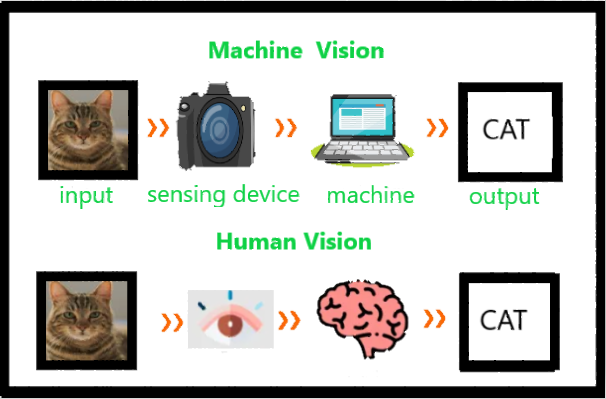
\includegraphics[scale=0.3]{./Figures/mv_comp.png}
	\caption{Componentes de un sistema de vision artificial y un sistemad de vision humano.}
	\label{fig:mv_comp}
\end{figure}

% hablar de los campos de estudio %

\subsection{Deteccion facial}
Uno de los campos de estudio mas importantes de la vision artificial es la deteccion facial. La deteccion facial puede ser considerada como un caso particular de la deteccion de objetos y tiene los objetivos de detectar y localizar todos los rostros humanos contenidos en una imagen digital. En la figura \ref{fig:mv_fd} se puede observar una imagen procesada por un sistema de deteccion facial.

\begin{figure}[h]
	\centering
	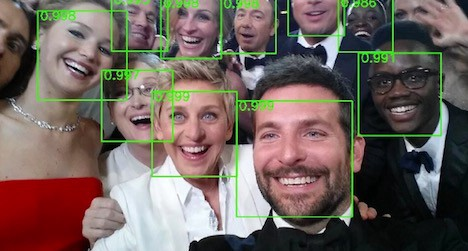
\includegraphics[scale=0.5]{./Figures/mv_fd.jpeg}
	\caption{Imagen procesada por un sistema de deteccion facial.}
	\label{fig:mv_fd}
\end{figure}

Hoy en dia, muchos dispositivos comerciales y profesionales como smartphones, tablets y robots, utilizan la deteccion facial como primer paso para otro tipo de aplicaciones mas complejas, entre las que destacan: reconocimento facial, computacion afectiva y grabacion de video inteligente.

\subsection{Vision artificial embebida}


%----------------------------------------------------------------------------------------
\section{Servicios en la nube}
El termino servicios en la nube hace referencia a un amplio rango de servicios ofrecidos bajo demanda a companias y usuarios a traves de internet. Estos servicios estan disenados para proveer de una manera facil y asequible acceso a aplicaciones y recursos, sin la necesidad de una infrastructura o hardware propios.

Los servicios en la nube son administrados totalmente por proveedores de computacion en la nube [ref]. Estos se encuentran disponibles para los usuarios desde los servidores de los proveedores, por lo que no es necesario que una empresa aloje aplicaciones en sus propios servidores.

De manera general, existen tres tipos basicos de servicios en la nube [ref]:

\begin{itemize}
	\item SaaS (\textit{Software as a Service}, Software como un Servicio): en este servicio el proveedor solo proporciona el software o aplicaciones en la nube mediante internet. Los clientes tienen acceso a traves de APIs (\textit{Application Programming Interface}, Interfaz de Programacion de Aplicaciones) o a traves de la web, que les permite interactuar de manera sencilla, sin la necesidad de gestionar, instalar ni actulizar el software. 
	\item IaaS (\textit{Infrastructure as a Service}, Infrastructura como un Servicio): este servicio implica la contatacion de una infraestructura de hardware a un tercero, donde varios cliente comparten los recursos de una maquina fisica. El proveedor proporciona a sus clientes el acceso a los recursos computacionales necesarios para almancenar o ejecutar tareas que pueden incluir servidores, redes, \textit{backup}, \textit{firewalls}, entre otros.
	\item PaaS (\textit{Platform as a Service}, Plataforma como un Servicio): es un servicio que se encuentra conceptualmente entre SaaS e IaaS al eliminar la parte fisica de la infraestructura y ofrece una plataforma donde los cliente pueden crear, desarrollar, gestionar y distribuir sus aplicaciones. El proveedor es el encargado de la gestion y mantenimiento de la plataforma y permite que los clientes se dediquen exclusivamente en el desarrollo.
\end{itemize}

En la figura \ref{fig:cloud_services} se puede observar las diferencias entre estos servicios en funcion de los elementos que pueden gestionar.

\begin{figure}[h]
	\centering
	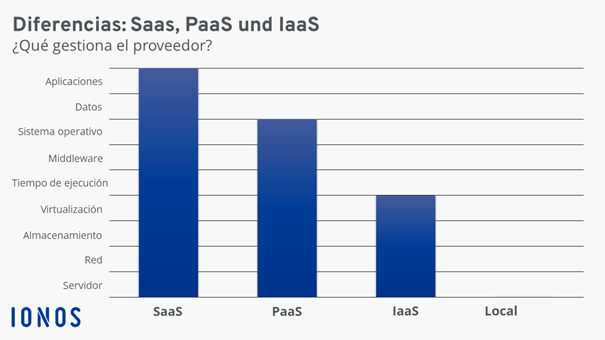
\includegraphics[scale=0.55]{./Figures/cloud_services.png}
	\caption{Capacidades de SaaS, IaaS y PaaS\protect\footnotemark.}
	\label{fig:cloud_services}
\end{figure}
\footnotetext{Imagen tomada de: \url{https://expansionba.com.ar/2020/05/23/medidas-para-amortiguar-el-costo-energetico-en-pymes/}}


%----------------------------------------------------------------------------------------
\section{Motivacion}
Gracias a la amplia gama de platarformas de hardware y la disponibilidad de bibliotecas de codigo abierto para implementar AI, ML y DL, ademas de la difusion de informacion en foros y sitios web especializados, es posible desarrollar sistemas de vision artificial personalizados para distintos tipos de arquitecturas [nwengineeringllc.com/article/computer-vision-in-embedded-systems-and-ai-platforms.php]. 

Estas bibliotecas de codigo para implementar vision artificial no suelen ser aptas para cualquier dispositivo, ya que son, en la mayoria de los casos, muy grandes en tamano y requieren de una capacidad de procesamiento lo suficientemente grande para ejecutarse en tiempo real. Pero los constantes esfuerzos de las empresas para ofrecer \textit{frameworks} optmizados que reducen el tamano y poder de procesamiento necesarios para ejecutar estos algoritmos, la integracion de aceleradores de hardware para redes neuronales y DSP (\textit{Digital Signal Processor, Procesador Digital de Senales}) en SoCs actuales (\textit{System on a Chip}, Sistema en un Chip) y el estudio de nuevas y mejoradas arquitecturas para vision artificial basadas en CNN, permiten el desarrollo de dispositivos emebebidos con la capacidad de ejecutar modelos de vision artificial. Algunas de sus aplicaciones mas importantes son: industria 4.0, seguridad, vehiculos autonomos y robotica.

La motivacion principal de este trabajo fue desarrollar un sistema embebido de bajo costo economico, bajo consumo energetico y de codigo abierto, que integre algoritmos de DL para vision artificial enfocado a la tarea de deteccion facial.

Una motivacion adicional fue integrar otra tecnologia actual como es IoT (\textit{Internet of Things}, Internet de las Cosas), para trabajar en conjunto con los algoritmos de vision artificial. Asi las aplicaciones que se pueden obtener son mas versatiles a la hora de su implementacion en entornos urbanos. 

%----------------------------------------------------------------------------------------
\section{Estado del arte}
Como antecedente existe un trabajo denominado "A New IoT Combined Face Detection of People by Using Computer Vision for Security Application" de ... El \textit{paper} donde se describe su trabajo presenta el desarrollo de un dispositivo electronico que tiene como componentes principales una Raspberry Pi 3, un sensor PIR (\textit{Passive Infra Red}, Pasivo Infra Rojo) y una camara. Su objetivo principal es detectar personas con ayuda del sensor de movimiento PIR, fotografiarlas y aplicar el algoritmo de deteccion facial Haar Cascade [ref], para posteriormente guardar una imagen del rostro detectado y visualizarla en un telefono movil con ayuda de la aplicacion Telegram. En la figura \ref{fig:soa_arch} se puede observar el diagrama en bloques del sistema descrito anteriormente.

\begin{figure}[h]
	\centering
	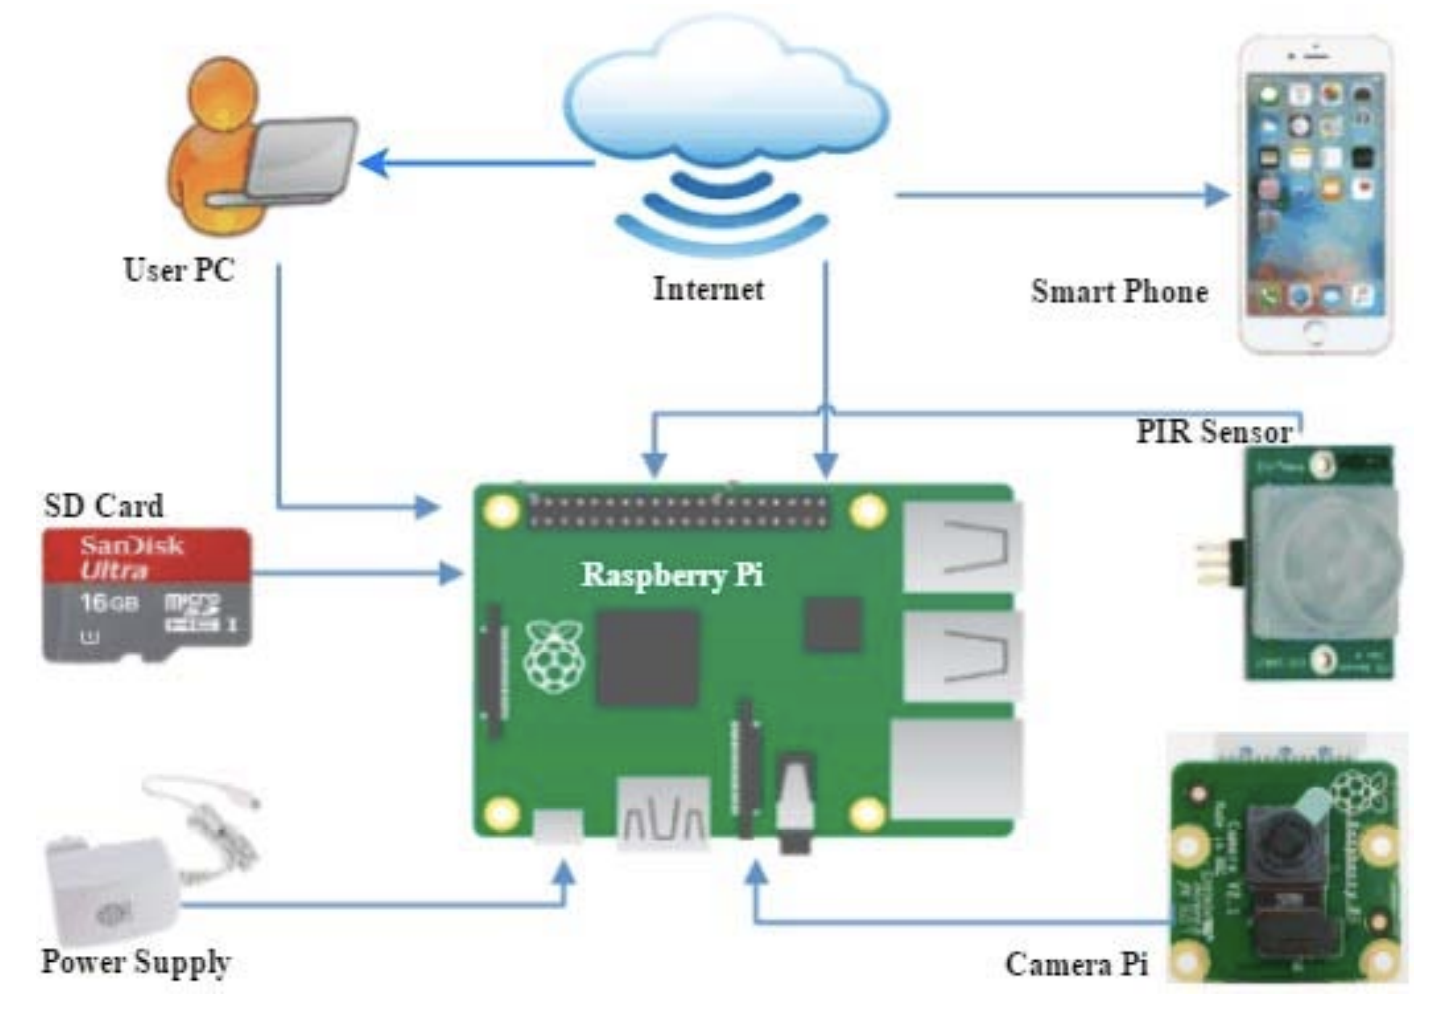
\includegraphics[scale=0.3]{./Figures/soa_arch.png}
	\caption{Imagen procesada por un sistema de deteccion facial.}
	\label{fig:soa_arch}
\end{figure}

%----------------------------------------------------------------------------------------
\section{Objetivos y alcance}
El objetivo principal de este trabajo fue desarrollar un sistema embebido con la capacidad de ejecutar modelos de AI para detectar y localizar rostros humanos de imagenes digitales capturadas por su camara.

El alcance de este trabajo incluyo:
\begin{itemize}
	\item Construccion de un prototipo de pruebas
	\item Desarrollo e implementacion de los modelos de AI necesarios
	\item Implementacion de los servicios en la nube necesarios
\end{itemize}
%----------------------------------------------------------------------------------------
\section{Requerimientos}



%----------------------------------------------------------------------------------------
